% !TEX root = main.tex
\chapter{The Powered Descent Guidance Problem}
\label{mathchapter}


\subsection{Dynamics}
In our formulation, the vehicle is treated as a rigid body. We assume that aerodynamic forces are negligible but that the body is subject to planetary gravitation $\mathbf{g}_I$. The algorithm as presented in \cite{} has the vehicle actuated by a single gimbaled thruster at the bottom of the vehicle. This engine has feasible thrust magnitude and efficiency, as well as standard gimbal range for agile vehicles. Modifications can be made here to include other actuators in the dynamics. I could have adapted my own actuator dynamics here, but to save time I have implemented the original algorithm.

We also capture mass depletion dynamics, proportional to the magnitude of the thrust generated by the engine. For tractability, we assume that the inertia matrix and the position of the center-of-mass is constant throughout the trajectory. We use the constant $\alpha_{\dot{m}}$, a function of the specific impulse, as the mass depletion parameter. Therefore we have that
\begin{align}
& \alpha_{\dot{m}} = \frac{1}{I_{sp} g_0} \\
& \dot{m}(t) = -\alpha_{\dot{m}} \left\lVert \mathbf{T}_B{t} \right\rVert _2
\end{align}

We will express the translational dynamics and forces acting on the vehicle in the inertially fixed frame. They are as follows:

\begin{align}
& \dot{\mathbf{r}}_I(t) = \mathbf{v}_I(t) \\
& \dot{\mathbf{v}}_I(t) = \frac{\mathbf{F}_I}{m(t)} + \mathbf{g}_I
\end{align}

The attitude formalism used in the paper are Euler parameters, or quaternions. They are used to denote the attitude of the vehicle between the $\mathcal{F}_B$ and $\mathcal{F}_I$ frames, $q_{B/I}(t)$ on the unit sphere. We use the angle-axis form of the quaternion, noted here:

\begin{align}
q_{B/I}(t) \triangleq 
	\begin{bmatrix}
	\cos(\phi/2) \\ \hat{n}\sin(\phi/2)
	\end{bmatrix}
	= 
	\begin{bmatrix}
	q_1 \quad q_2 \quad q_3 \quad q_4
	\end{bmatrix}^T
\end{align}

The $\hat{n} \in \mathcal{R}^3$ vector is the euler vector in which the single angle $\phi$ displaces the attitude about. In our derivation we will also need the direction cosine matrix produced by this quaternion. DCMs are part of the $SO(3)$ group with properties that its determinant is 1 and can be transposed/inverted for the reverse mapping. They can be multiplied to encode multiple rotations. The mapping from inertial to body frame is the following:

\begin{align}
C_{B/I}={\begin{bmatrix}1-2(q_{2}^{2}+q_{3}^{2})&2(q_{1}q_{2}-q_{0}q_{3})&2(q_{0}q_{2}+q_{1}q_{3})\\2(q_{1}q_{2}+q_{0}q_{3})&1-2(q_{1}^{2}+q_{3}^{2})&2(q_{2}q_{3}-q_{0}q_{1})\\2(q_{1}q_{3}-q_{0}q_{2})&2(q_{0}q_{1}+q_{2}q_{3})&1-2(q_{1}^{2}+q_{2}^{2})\end{bmatrix}}
\end{align}

In our attitude dynamics, we will use $\bm{\omega}_B(t) \in \mathcal{R}^3$ to denote the angular velocity vector of the vehicle in the $\mathcal{F}_B$ frame with respect to $\mathcal{F}_I$. The torque acting on the vehicle is written as $\mathbf{M}_B(t) \in \mathcal{R}^3$ in the body frame. We also use the $\left[\mathbf{r}^\times \right]$ operator to denote the skew symmetric form of the vector $\mathbf{r}$. The inertia tensor instantiated in $\mathcal{F}_B$ is written as $J_B \in \mathcal{R}^{3\times 3}$.

Given that we have chosen quaternions as our formalism, we must understand the kinematics as such:

\begin{align}
 & \dot{q}_{B/I}(t) = \frac{1}{2} B(\bm{\omega_B}(t)) q_{B/I}(t)
\end{align}

where the matrix $B(\bm{\omega_B}(t))$ is defined as 
\begin{align}
& B(\bm{\omega_B}(t)) = 
	\begin{bmatrix}
	0 & -\omega_1 & -\omega_2 & -\omega_3\\ 
	\omega_1 & 0 & \omega_3 & -\omega_2 \\
	\omega_2 & -\omega_3 & 0 & \omega_1 \\
	\omega_3 & \omega_2 & -\omega_1  & 0  \\
	\end{bmatrix}
\end{align}

We can also derive the simplified angular dynamics as the following
\begin{align}
& J_B \dot{\bm{\omega}}_B(t) = -\left[\bm{\omega}_B ^ \times\right] J_B \bm{\omega}_B + \mathbf{M}_B(t)
\end{align}
With the torque applied to the spacecraft.


\subsection{Constraints and Boundary Conditions}
We must now state the constraints and boundary values for the problem required by the optimization.
We know that we can never use more fuel than we have, therefore the convex constraint is 
\begin{align}
& m(t) \geq m_{dry}
\end{align}

Additionally we want to apply a glide slope constraint in the case that our vehicle has terrain relative navigation sensors. We form the convex constraint using the angle $\gamma_{gs}$:
\begin{align}
& \mathbf{e}_1 \cdot \mathbf{r}_I(t) \geq \tan(\gamma_{gs}) \left\lVert \left[\mathbf{e}_2 \quad \mathbf{e}_3\right]^T \mathbf{r}_I(t) \right\lVert_2
\end{align}
This effectively draws an upward facing cone slope that the vehicle must not penetrate. This type of convex constraint can also be useful in avoiding rocky terrain and enforcing a landing from directly above an area, minimizing lateral movement close to the ground.
The author also included that the vehicle must avoid excessive tilt angles such that it stays relatively upright throughout the trajectory, we can constrain a portion of the direction cosine matrix as such:
\begin{align}
& \cos(\theta_{max}) \leq 1-2(q_{2}^{2}+q_{3}^{2})
\end{align}

Along the same line of thought, we can constrain the angular rate using convex constraints as well:
\begin{align}
& \left \lVert \bm{\omega}_B(t) \right \lVert_2 \leq \omega_{max}
\end{align}

Finally we must encode that the commanded thrust vector needs to be constrained between two magnitudes, which is appropriate. We assume that the engine cannot be re-lit during operation (commonly becoming a bad assumption to make). We also know that there is some limit to the amount of gimbal angle we can perform $\delta_{max}$.
\begin{align}
& 0 < T_{min} \leq \left \lVert \bm{T}_B(t) \right \lVert_2 \leq T_{max} \\
& \cos(\delta_{max}) \left \lVert \bm{T}_B(t) \right \lVert_2 \leq \bm{e}_1 \cdot \bm{T}_B(t)
\end{align}

We see that the upper thrust bound is clearly convex but the lower bound creates a non-convex constraint. Because of the range of  $\delta_{max}$ turns out to be convex.

For the powered descent guidance problem, the boundary conditions are trivial to identify. The initial mass, position, velocity, attitude, and angular rates are given by the navigation subsystem at the moment in time. We assume the dry mass is known and that and estimate of the wet mass can be backed out. The terminal position is the landing site. The terminal translational and angular velocities can be zero, with the terminal attitude in the upright position. The final mass should be free. The initial thrust vector should be free, while the terminal vector should be along the vehicle up, X-axis. The author intends on the initial attitude being free, which can free up the optimization for shorter final times.




\subsection{Continuous Time Problem}
Putting this all together we can pose the continuous time optimization problem. In this form, it is non-convex and requires significant conditioning to work into the convex framework. As stated, the objective is to minimize the time-of-flight required to get to the terminal conditions subject to the aforementioned constraints, dynamics, and boundary conditions. We leave the commanded thrust, gimbal angles, and final time free. It is as follows:
\clearpage

\begin{mdframed}
\textbf{Problem 1: Continuous Time Non-Convex Free-Final-Time}

\underline{Cost Function:}
\begin{equation*}
\min_{\mathbf{T}_B, t_f} t_f
\end{equation*}

\underline{Boundary Conditions:}  
\begin{align*}
& m(0) = m_{wet} \quad \mathbf{r}_I(0) = \mathbf{r}_i \quad \mathbf{v}_I(0) = \mathbf{v}_i \quad \quad \quad{q}_{B/I}(0) = {q}_{B/I _{i}} \quad \bm{\omega}_B(0) = \bm{\omega}_{B _{i}} \\
& \mathbf{r}_I(t_f) = \mathbf{0} \quad \quad \mathbf{v}_I(t_f) = \mathbf{0} \quad {q}_{B/I}(t_f) = {q}_{B/I _ {f}} \quad \bm{\omega}_B(t_f) = \mathbf{0} \\
& \mathbf{e}_2 \cdot \mathbf{T}_B(t_f) = \mathbf{e}_3 \cdot \mathbf{T}_B(t_f) = 0
\end{align*}

\underline{Dynamics:}  
\begin{align*}
& \dot{m}(t) = -\alpha_{\dot{m}} \left\lVert \mathbf{T}_B{t} \right\rVert _2 \\
& \dot{\mathbf{r}}_I(t) = \mathbf{v}_I(t) \\
& \dot{\mathbf{v}}_I(t) = \frac{C_{I/B}(t)\mathbf{T}_B(t)}{m(t)} + \mathbf{g}_I \\
 & \dot{q}_{B/I}(t) = \frac{1}{2} B(\bm{\omega_B}(t)) q_{B/I}(t) \\
& J_B \dot{\bm{\omega}}_B(t) = -\left[\bm{\omega}_B ^ \times\right] J_B \bm{\omega}_B + \left[r_{com}^\times \right]\mathbf{T}_B(t)
\end{align*}

\underline{State Constraints:}  
\begin{align*}
& m(t) \geq m_{dry} \\
& \mathbf{e}_1 \cdot \mathbf{r}_I(t) \geq \tan(\gamma_{gs}) \left\lVert \left[\mathbf{e}_2 \quad \mathbf{e}_3\right]^T \mathbf{r}_I(t) \right\lVert_2 \\
& \cos(\theta_{max}) \leq 1-2(q_{2}^{2}+q_{3}^{2}) \\
& \left \lVert \bm{\omega}_B(t) \right \lVert_2 \leq \omega_{max}
\end{align*}

\underline{Control Constraints:}  
\begin{align*}
& 0 < T_{min} \leq \left \lVert \bm{T}_B(t) \right \lVert_2 \leq T_{max} \\
& \cos(\delta_{max}) \left \lVert \bm{T}_B(t) \right \lVert_2 \leq \bm{e}_1 \cdot \bm{T}_B(t)
\end{align*}

\end{mdframed}


























% The objective of this fake thesis document is to demonstrate
% a multitude of \LaTeX{} features as well as features specific
% to the thesis class.
% We start by giving one short formula,
% and one big hairy multi-line formula
% (one of the non-dimensional Navier-Stokes equations):

% \begin{equation}
% 	A = \pi r^2
% \end{equation}


% \begin{eqnarray}
%   \rho \left[ \frac{DV_r}{Dt} - M \epsilon^2
%     \frac{\vth^2}{r} \right]
%   & = & -\frac{\delta^2}{\gamma~ M} \diffr{P}
% 	+ \frac{M ~\delta^2}{Re} \left\{ 2 \diffr{}
% 	\left[ \mu \left( \diffr{V_r}
%         - \frac{1}{3} {\bf \nabla \cdot \overline{V}}
%       \right) \right] \right. \nonumber \\
%   & & + \frac{1}{r} \diffth{} \left[ \mu \left(
%       \frac{1}{r} \diffth{V_r} + \epsilon \diffr{\vth}
%       - \epsilon \frac{\vth}{r} \right) \right] \nonumber \\
%   & & + \diffz{} \left[ \mu \left( \frac{1}{\delta^2}
%         \diffz{V_r} + \diffr{V_z} \right) \right] \nonumber \\
%   & & + 2 \left. \frac{\mu}{r}\left[ \diffr{V_r} -\frac{\epsilon}{r}
%       \diffth{\vth} - \frac{V_r}r\right] \right\}, \label{eq:rmom}
% \end{eqnarray}


% \section{Explanation of equations}

% The latter equation is non-dimensionalized using the following definitions:

% \[
% 	r = \frac{r'}{R'}, ~~~
% 	z = \frac{z'}{L'},~~~
% 	t = \frac{t'}{t_a'}, ~~~
% 	\kappa = \frac{\kappa'}{\kappa_0'}, ~~~
% 	\mu = \frac{\mu'}{\mu_0'} , ~~~
% 	C_V = \frac{C_V'}{C_{V0}'},
% \]
% where $P_0'$ is the initial static pressure in the cylinder,
% and $\rho_0'$ and $T_0'$ are the density and temperature
% of the fluid being injected from the sidewall.

% \begin{figure}[htbp]
%     \caption[Cutting up a triangular pyramid]{
% 	A triangular pyramid may be cut up as shown, to
% 	yield one top pyramid (with one-eighth the volume
% 	of the full pyramid), three bottom corner pyramids
% 	(which, when joined, are congruent to the top pyramid),
% 	three prisms along the bottom edges (the area of whose
% 	bottom faces total $B/2$) and the large central prism
% 	(volume = $(B/4)(h/2) = Bh/8$).
% 	The image, from PDF file ``pyr.pdf'',
% 	was read in using the {\tt $\backslash$includegraphics}
% 	command, from the {\tt graphicx} package.
% 	}
%     \begin{center}
% 	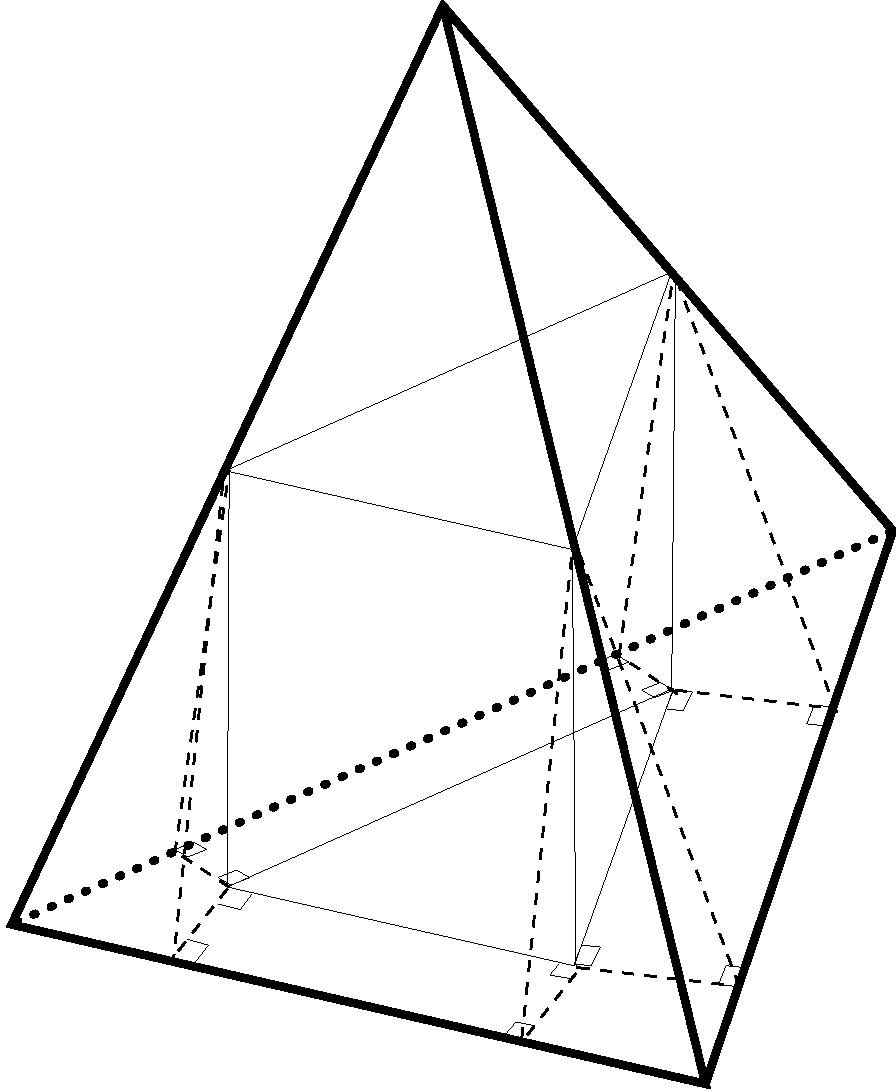
\includegraphics[width=90mm]{figs/pyr.pdf}
%     \end{center}
% \label{pyramid}
% \end{figure}


% Here is an example of using the macros
% \verb2\singlespacing2 and \verb2\doublespacing2:

% \singlespacing	% <------------------------------

% This paragraph was preceded by the
% command \verb2\singlespacing2.
% See the Specifications of the Grad School for instructions
% about when single spacing is appropriate in a thesis.

% \doublespacing	% <------------------------------

% And now, here is an example of using the macros
% \verb2\begin{singlespace}2 and \verb2\end{singlespace}2;
% another way to get single-spacing.

% \begin{singlespace}	% <-----------------------------
% Two cases are studied in the present work which differ only in the
% boundary conditions.  Each different boundary condition model a
% different source of instability.  The boundary of the first case
% consists of a steady, axisymmetric sidewall radial velocity boundary
% and a time-dependent, non-axisymmetric endwall axial velocity
% boundary.  The second case is studied with a fixed impermeable axial
% velocity along the endwall and a combination axisymmetric steady and
% non-axisymmetric unsteady radial velocity along the sidewall.
% \end{singlespace}	% <-----------------------------


% Usually you want to use a table produced by some other
% software, such as Excel, rather than try to do it using
% \LaTeX macros.  If the table is saved/printed to a PDF file,
% then it can be displayed using the
% $\backslash${\tt includegraphics} macro
% inside a {\tt table} environment:


% \begin{table}
%     \caption[Table from a PDF file]{
% 	This table wasn't constructed with \LaTeX{}
% 	commands, but resides in PDF file
% 	({\tt tableD.pdf})
% 	created by some other software.
% 	}
%     \begin{center}
% 	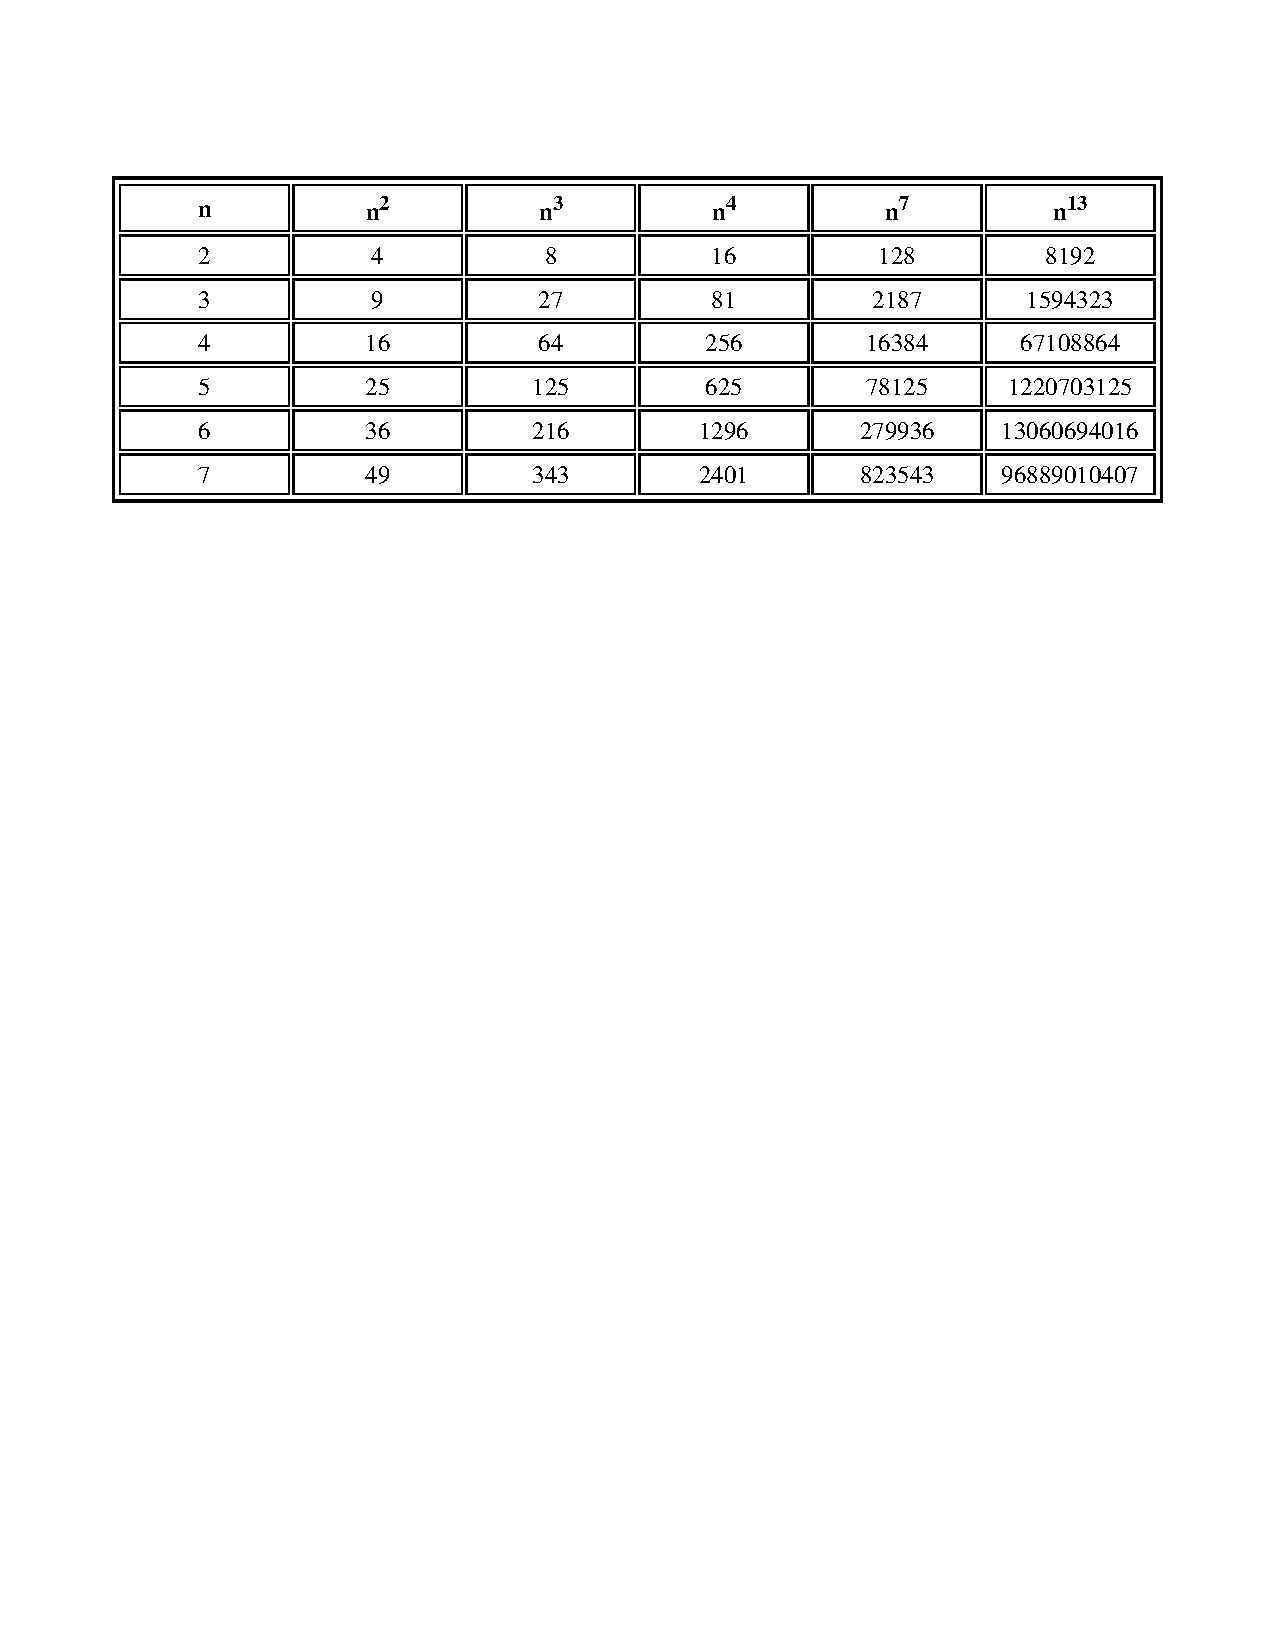
\includegraphics[width=5.45in]{figs/tableD.pdf}
%     \end{center}
% \label{pdftable}
% \end{table}


% Some of the boundary conditions are:

% \begin{eqnarray}
%   z=0; && V_z = \twochoices
% 	{0, && t\leq0}
% 	{\widetilde{F}_{zw}(r,\theta,t), && t>0}
% 						\label{eq:endwall} \\
%   z=0; && V_{\theta}=V_r=0			\label{eq:endnoslip} \\
%   r=0; && P,\rho,T,V_r,\vth,V_z~\mbox{finite},	\label{eq:centerline} \\
%   r=1; && V_r= F_{rws}(z),			\label{eq:injection} \\
%   r=1; && V_z=\vth =0,				\label{eq:sidenoslip}
% \end{eqnarray}
% and solutions must be periodic in $\theta$.

% If you don't believe this stuff, check out
% Mulick\cite{mulick} and Baylor\cite{baylor}.


% \section{Yet another section}

% \subsection{
% 	Just meaningless text to test lines per page
% 	\label{ss}}

% According to the Grad School specs.   there should be 24--27 lines
% of print per page of a thesis.  This should be true whether the font
% size is 10, 11, or 12.  Count them up; does this document conform?
% According to the Grad School specs.   there should be 24--27 lines
% of print per page of a thesis.  This should be true whether the font
% size is 10, 11, or 12.  Count them up; does this document conform?
% According to the Grad School specs.   there should be 24--27 lines
% of print per page of a thesis.  This should be true whether the font
% size is 10, 11, or 12.  Count them up; does this document conform?
% According to the Grad School specs.   there should be 24--27 lines
% of print per page of a thesis.  This should be true whether the font
% size is 10, 11, or 12.  Count them up; does this document conform?
% According to the Grad School specs.   there should be 24--27 lines
% of print per page of a thesis.  This should be true whether the font
% size is 10, 11, or 12.  Count them up; does this document conform?
% According to the Grad School specs.   there should be 24--27 lines
% of print per page of a thesis.  This should be true whether the font
% size is 10, 11, or 12.  Count them up; does this document conform?
% According to the Grad School specs.   there should be 24--27 lines
% of print per page of a thesis.  This should be true whether the font
% size is 10, 11, or 12.  Count them up; does this document conform?
% According to the Grad School specs.   there should be 24--27 lines
% of print per page of a thesis.  This should be true whether the font
% size is 10, 11, or 12.  Count them up; does this document conform?
% According to the Grad School specs.   there should be 24--27 lines
% of print per page of a thesis.  This should be true whether the font
% size is 10, 11, or 12.  Count them up; does this document conform?
% According to the Grad School specs.   there should be 24--27 lines
% of print per page of a thesis.  This should be true whether the font
% size is 10, 11, or 12.  Count them up; does this document conform?
% According to the Grad School specs.   there should be 24--27 lines
% of print per page of a thesis.  This should be true whether the font
% size is 10, 11, or 12.  Count them up; does this document conform?
% According to the Grad School specs.   there should be 24--27 lines
% of print per page of a thesis.  This should be true whether the font
% size is 10, 11, or 12.  Count them up; does this document conform?
% According to the Grad School specs.   there should be 24--27 lines
% of print per page of a thesis.  This should be true whether the font
% size is 10, 11, or 12.  Count them up; does this document conform?
% According to the Grad School specs.   there should be 24--27 lines
% of print per page of a thesis.  This should be true whether the font
% size is 10, 11, or 12.  Count them up; does this document conform?
% According to the Grad School specs.   there should be 24--27 lines
% of print per page of a thesis.  This should be true whether the font
% size is 10, 11, or 12.  Count them up; does this document conform?
% According to the Grad School specs.   there should be 24--27 lines
% of print per page of a thesis.  This should be true whether the font
% size is 10, 11, or 12.  Count them up; does this document conform?
% According to the Grad School specs.   there should be 24--27 lines
% of print per page of a thesis.  This should be true whether the font
% size is 10, 11, or 12.  Count them up; does this document conform?

% \paragraph{What is it?}
% This is a labelled paragraph.
% The heading of the paragraph is emphasized.
% This is a labelled paragraph.
% The heading of the paragraph is emphasized.

% \subsection{This is a subsection}

% This is a subsection.
% Filler filler filler filler filler filler filler filler.
% Filler filler filler filler filler filler filler filler.

% \subsection{This is another subsection}

% This is another subsection.
% Filler filler filler filler filler filler filler filler.
% Filler filler filler filler filler filler filler filler.

% \paragraph{This is paragraph number 2.}
% It used a \verb2\paragraph{}2 header, which
% are always inlined (with extra space)
% and  boldfaced.

% This is the third paragraph of the subsection.
% Filler filler filler filler filler filler filler filler.
% Filler filler filler filler filler filler filler filler.

% %%%%%%%%%%%%%%%%%%%%%%%%%%%%%%%%%%%%%%%%%%%%%%%%%%%%%%%%%%

% \subsubsection{This is a subsubsection (1)}
% This is the first paragraph of the subsubsection.
% Whether it is numbered or inlined depends on the
% option selected at the beginning of the
% thesis.

% By default, a \verb2\subsubsection2 heading is numbered
% and set off on a separate line, left-justified.

% \paragraph{However.}
% Using the \verb2inlineh42 option, subsubsection headers
% are inlined.
% And using the \verb2nonumh42 option suppresses
% numbering of the subsubsections.
% Together they make subsubsection headings
% just the same as paragraph headings.


% %%%%%%%%%%%%%%%%%%%%%%%%%%%%%%%%%%%%%%%%%%%%%%%%%%%%%%%%%%

% \subsubsection{
% 	This is another subsubsection (2)
% 	\label{sss}
% 	}

% Once again, whether its heading is numbered
% and/or inlined depends on the class options
% chosen at the start.

% There is no ``subsubsubsection'' entity,
% and ``subparagraph'' gets no special treatment
% in \emph{thesis} class.

% \section{The End}
% \label{sec:end}

% Finally, this is the end.  The bibliography starts on
% the next page.
% Note how the \verb2\hyperref2 package
% (mentioned in chapter \ref{introchap})
% also makes hyperlinks from references
% (e.g., Mulick\cite{mulick})
% to entries in the bibliography.

